\subsection{mmap}
\subsubsection{内存映射}
内存映射,简而言之就是将用户空间的一段内存区域映射到内核空间,映射成功后,用户对这段内存区域的修改可以直接反映到内核空间,同样,内核空间对这段区域的修改也直接反映用户空间。
以下是一个把普遍文件映射到用户空间的内存区域的示意图。

\begin{figure}[H]
    \centering
    \caption[short]{内存映射}
    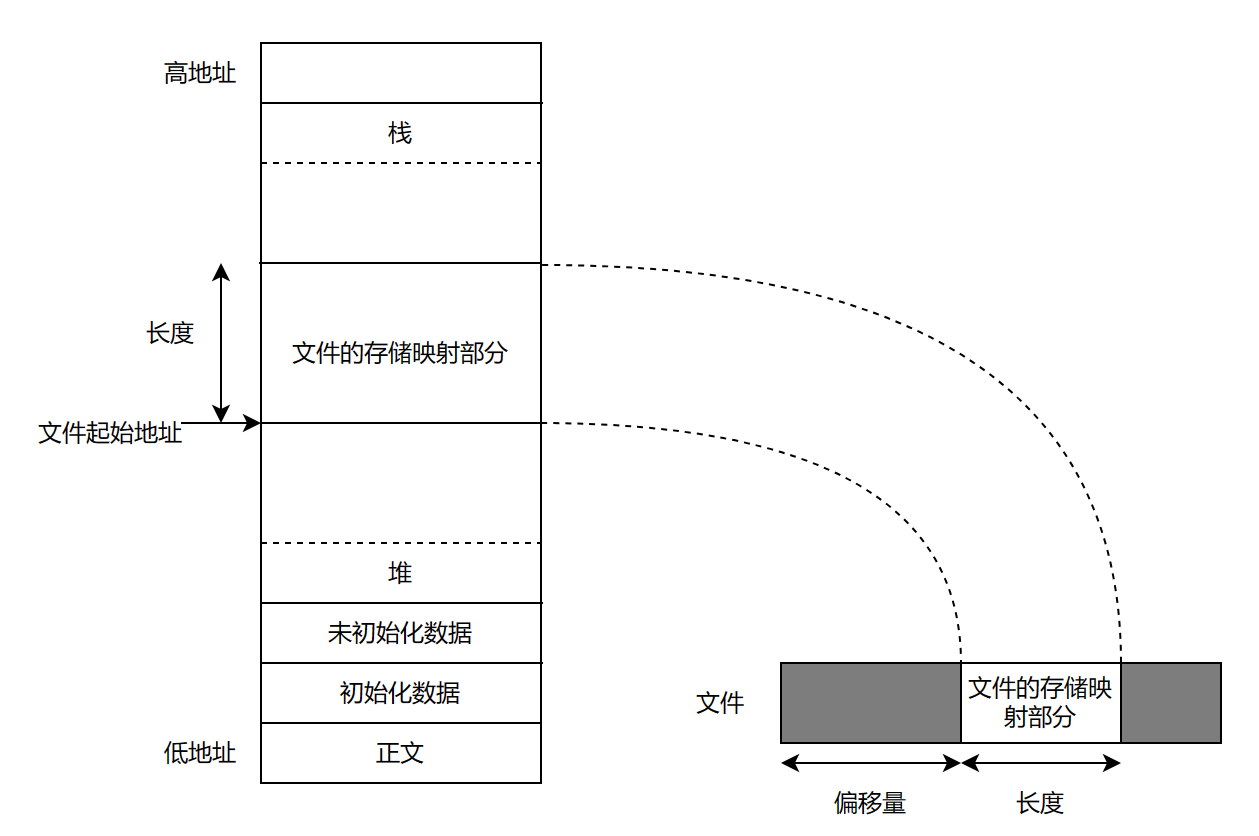
\includegraphics[width=0.8\linewidth]{figures/09-04-mmap-内存映射.png}
\end{figure}

\subsubsection{mmap主要用途}
\textbf{传统的读写文件}

一般来说,修改一个文件的内容需要如下3个步骤:把文件内容读入到内存中。修改内存中的内容。把内存的数据写入到文件中。

从传统读写文件的过程中,我们可以发现有个地方可以优化:如果可以直接在用户空间读写页缓存,那么就可以免去将页缓存的数据复制到用户空间缓冲区的过程。
那么,有没有这样的技术能实现上面所说的方式呢?答案是肯定的,就是mmap。

\textbf{使用mmap读写文件}

mmap用于把文件映射到用户空间中,简单说mmap就是把一个文件的内容在内存里面做一个映像。那么对于内核空间与用户空间两者之间需要大量数据传输等操作的效率是非常高的。进程可以像读写内存一样对普通文件的操作。
mmap系统调用也可以使得进程之间通过映射同一个普通文件实现共享内存。

该函数主要用途有三个:
\begin{enumerate}
    \item 将一个普通文件映射到内存中,通常在需要对文件进行频繁读写时使用,这样用内存读写取代I/O读写,以获得较高的性能;
    \item 将特殊文件进行匿名内存映射,可以为关联进程提供共享内存空间;
    \item 为无关联的进程提供共享内存空间,一般也是将一个普通文件映射到内存中。
\end{enumerate}

\subsubsection{mmap实现}
下面将结合NPUcore的代码来介绍mmap的实现

从上文可知,要实现mmap,就要实现用户空间到内核空间的内存映射。所以mmap会分别确定要映射的用户空间和内存空间。

\textbf{用户空间}

mmap会申请一块适合的虚拟内存作为待映射的用户空间
\begin{lstlisting}[language={Rust},
	caption={os/src/mm/memory_set.rs}]
let area: &mut MapArea = &mut self.areas[idx];
let start_va = area.inner.vpn_range.get_end()
let end_va = start_va + len;

let mut new_area: MapArea = MapArea::new(
    start_va,
    end_va,
    MapType::Framed,
    map_perm,
    map_file,
);
\end{lstlisting}
MapArea是一个描述虚拟地址的结构体,它指向某块用户空间的首尾,mmap在获取该结构体后会将其链入其进程管理的所有虚拟地址中。

\begin{figure}[H]
    \centering
    \caption[short]{虚拟地址结构体}
    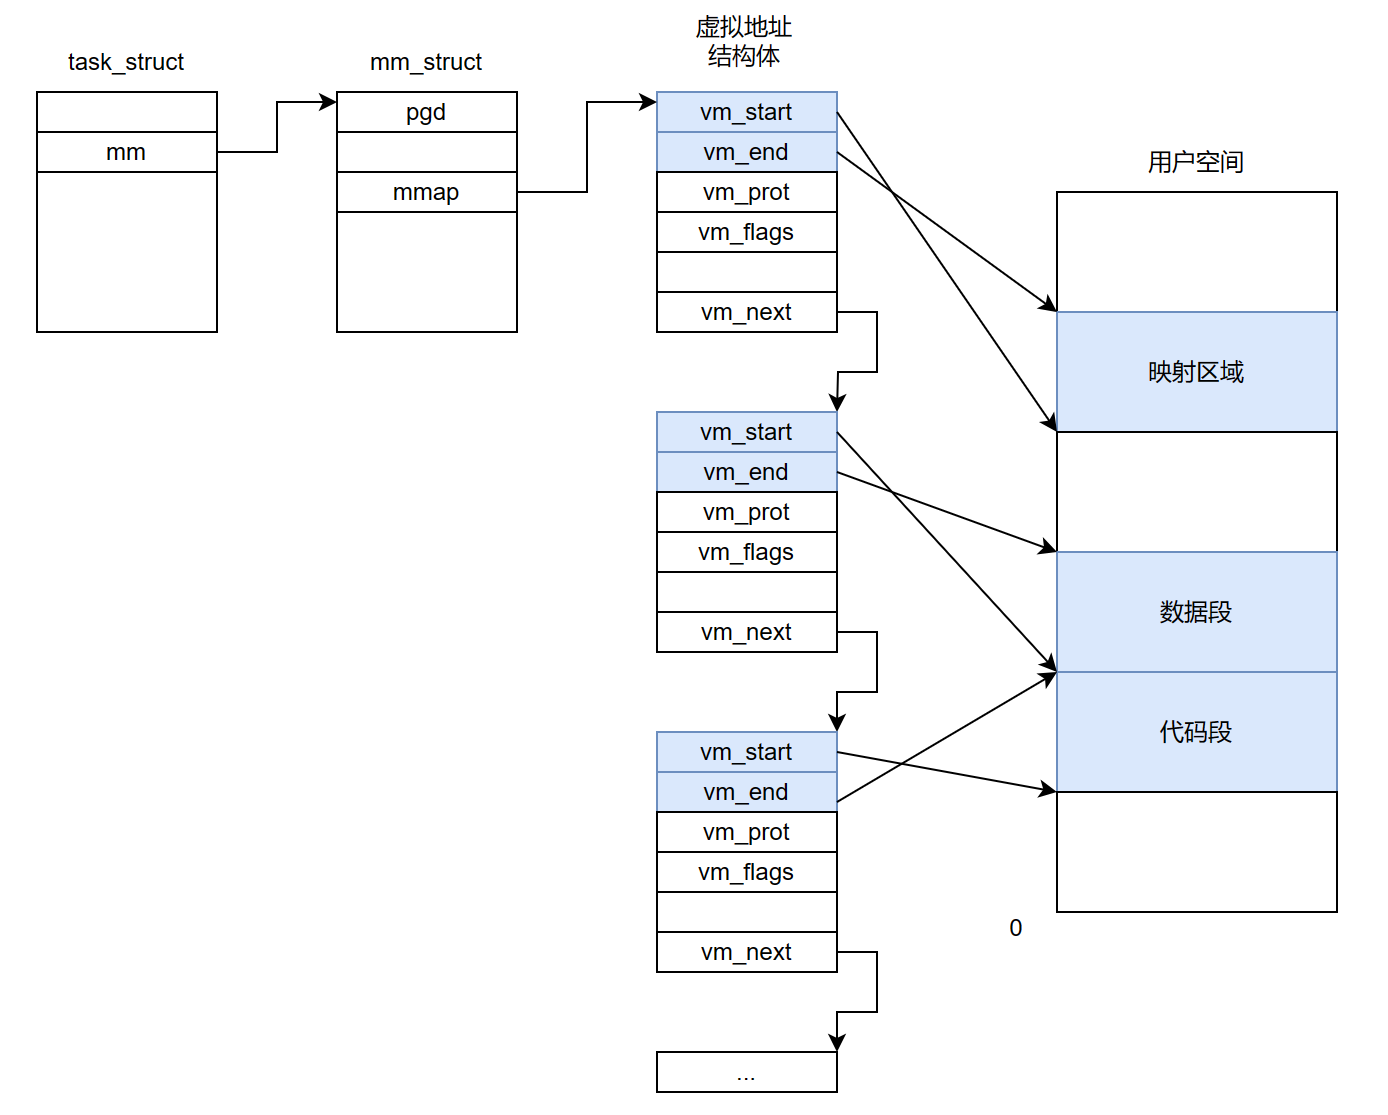
\includegraphics[width=0.8\linewidth]{figures/09-04-mmap-虚拟地址结构体.png}
\end{figure}

\textbf{内核空间}

mmap获取待映射的内核空间是通过进程打开的文件描述符获取的
\begin{lstlisting}[language={Rust},
	caption={os/src/mm/memory_set.rs}]
let fd_table = task.files.lock();
match fd_table.get_ref(fd) {
    Ok(file_descriptor) => {
        if !file_descriptor.readable() {
            return EACCES;
        }
        let file = file_descriptor.file.deep_clone();
        file.lseek(offset as isize, SeekWhence::SEEK_SET).unwrap();
        new_area.map_file = Some(file);
    }
    Err(errno) => return errno,
}
\end{lstlisting}
NPUcore中将文件对应的内核空间file存入了new\_area.map\_file中
这样既确定了要映射的用户空间和内存空间,也完成了它们之间的映射。

\textbf{其他}

mmap支持文件映射和匿名映射,如果是文件映射,则会通过上述的确定内核空间的过程,如果是匿名映射,那么该进程只是申请了一块空间,这片空间不与任何文件关联。

